\documentclass{article}

\usepackage{enumerate}
\usepackage{amssymb}
\usepackage{amsmath}
\usepackage{algorithm}
\usepackage[noend]{algpseudocode}
\usepackage{graphicx}
\usepackage{listings}

\graphicspath{ {Images/} }

\topmargin=-0.45in
\evensidemargin=0in
\oddsidemargin=0in
\textwidth=6.5in
\textheight=9.0in
\headsep=0.25in

\title{CS 189: Homework 6}
\author{Michael Stephen Chen\\ Kaggle Acct: michaelstchen \\SID: 23567341}

\begin{document}
\maketitle

\pagebreak

\section*{Problem 1}
The stochastic gradient descent update for the weights $V$ and $W$ are as follows,
$$V = V - \epsilon \nabla_V J$$
$$W = W - \epsilon \nabla_W J$$

Where $J$ is our loss function. The derivation for $\nabla_V J$ and $\nabla_W J$ when using the \textbf{mean squared error} as our loss function is provided below
\begin{center}
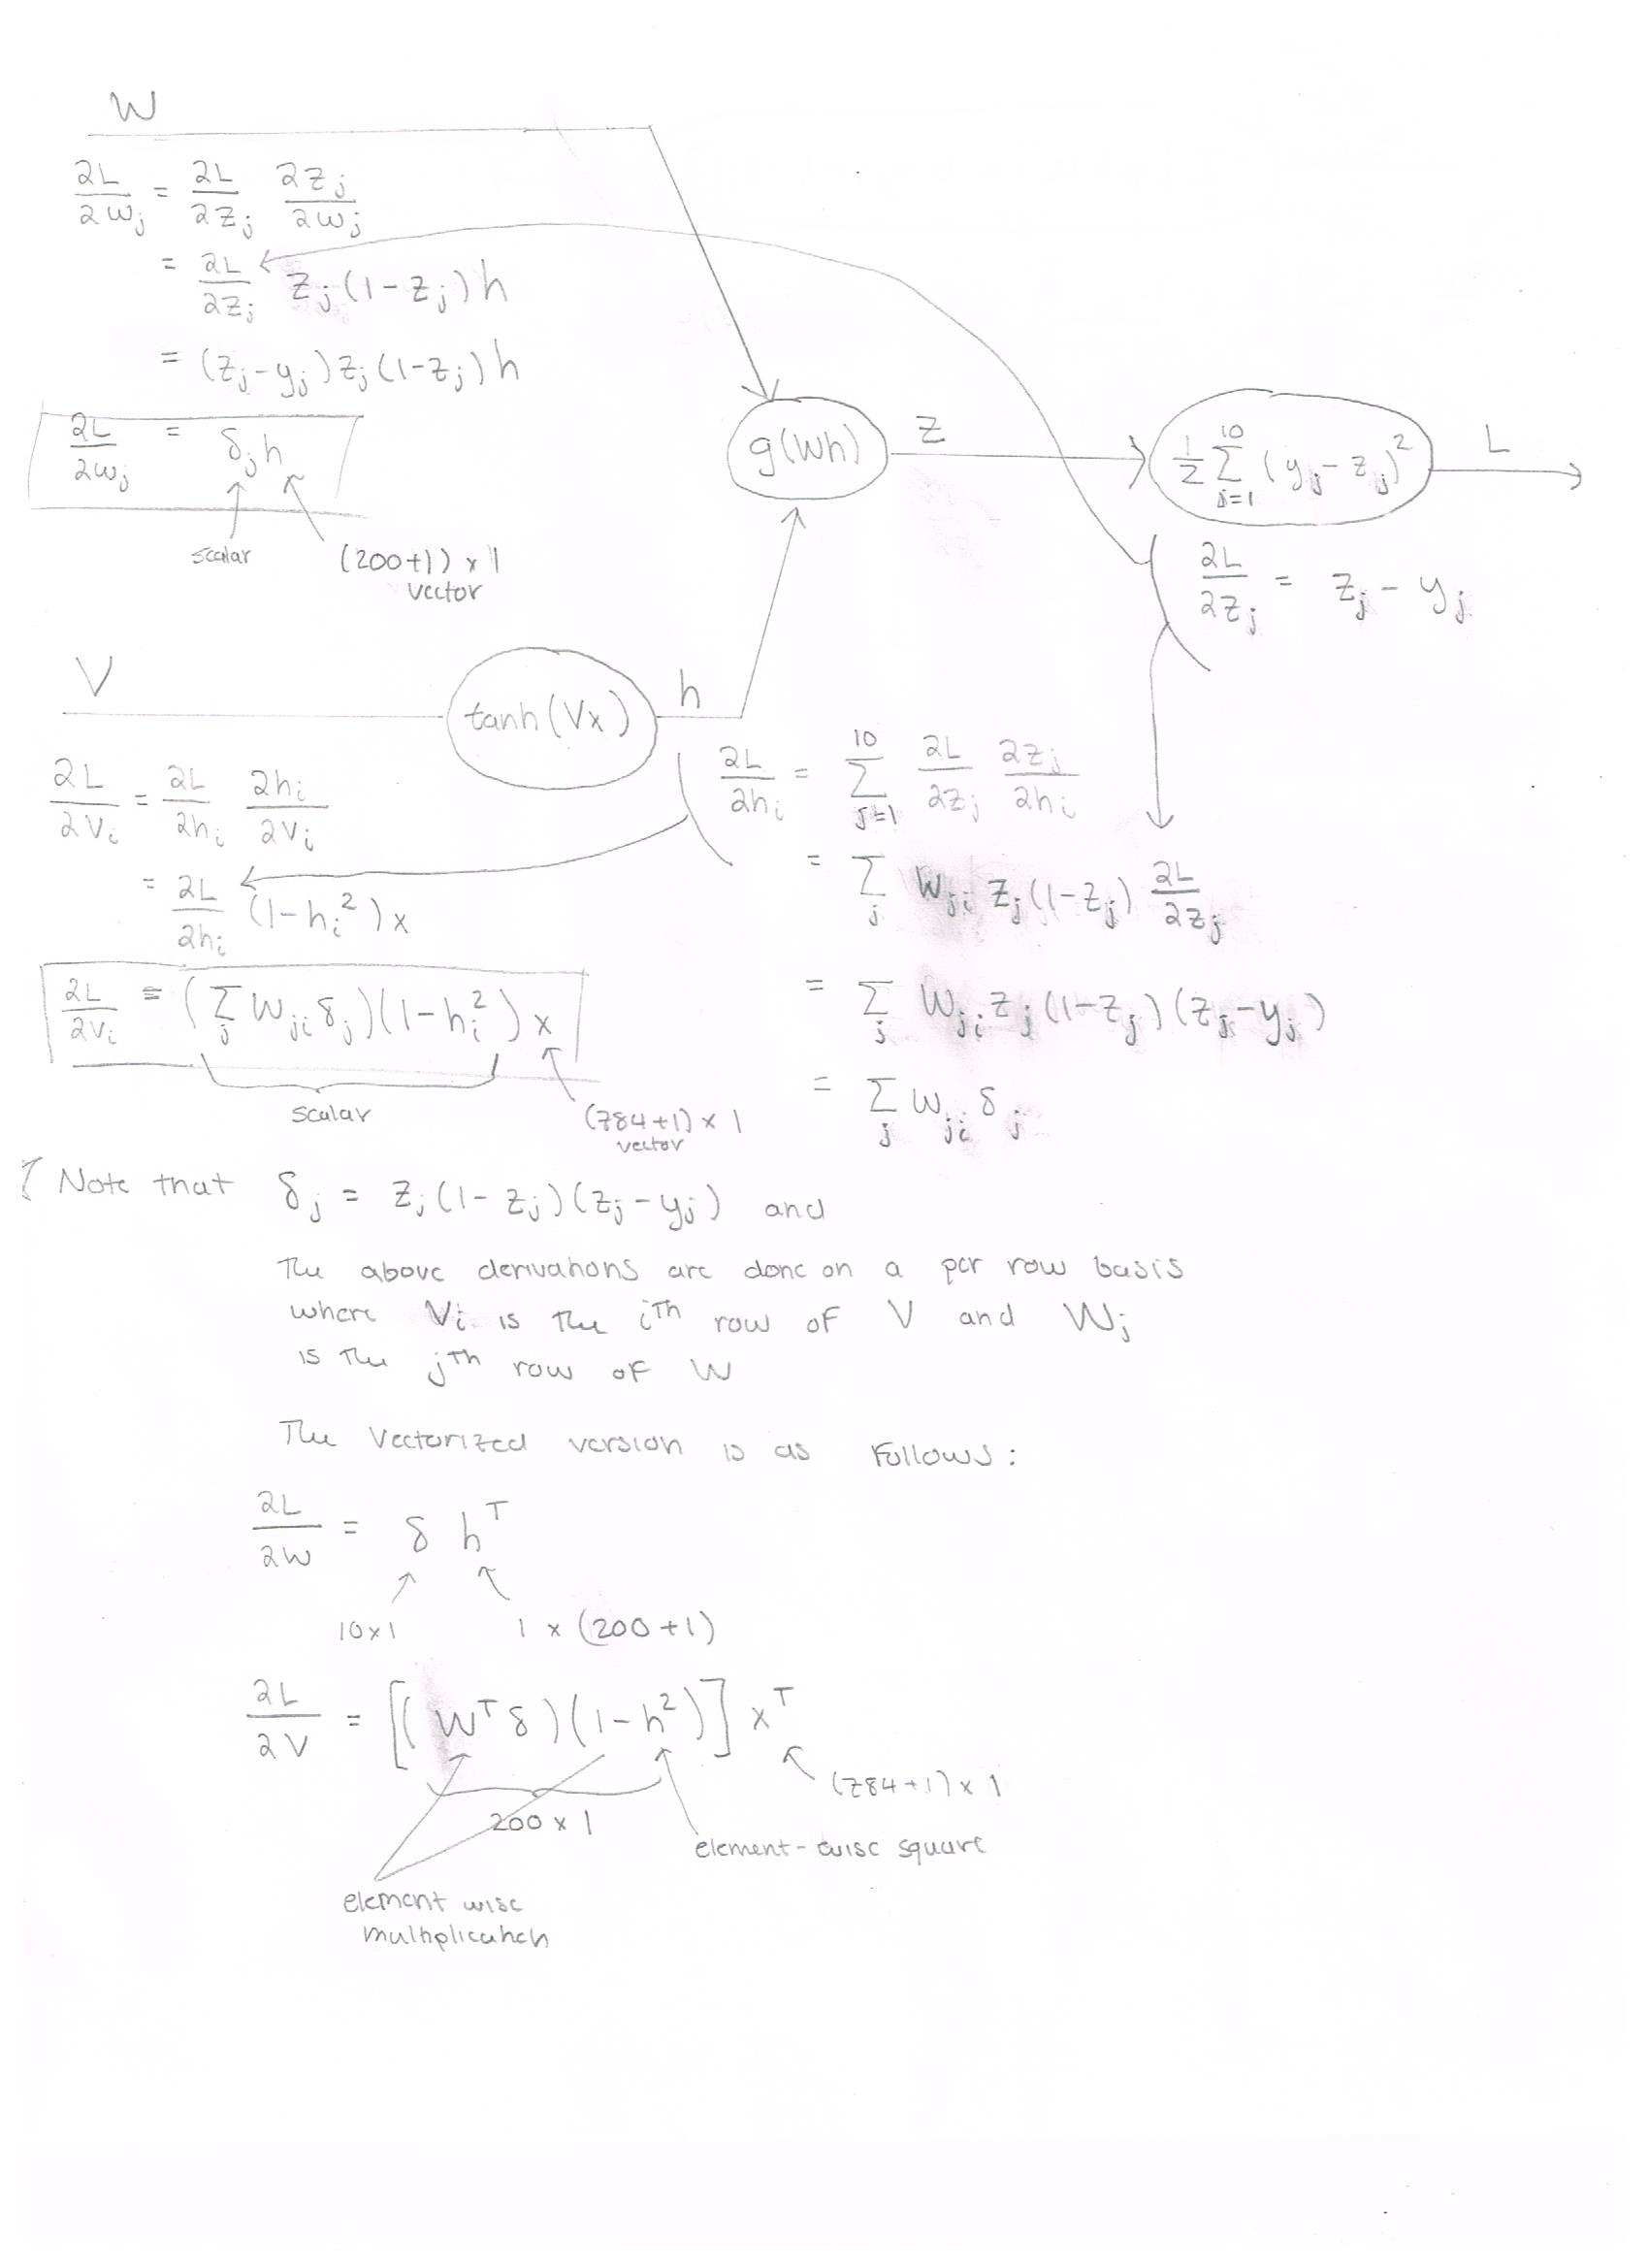
\includegraphics[scale=0.65]{001}
\end{center}

In the above derivation, I adjusted the indexing notation from what was given (please refer to the starred ``Note'' above). Also I use the same index $j$ to denote row $j$ of the $W$ matrix as well as to denote the $j^{th}$ element of the vectors $z_j$ and $y_j$ (so $1 \leq j \leq 10$). Likewise I use $i$ to denote the $i^{th}$ row of $V$ as well as the $i^{th}$ column of $W$ (so $1 \leq i \leq 200 or 201$). This is the indexing scheme that Prof. Shewchuck used in his lecture notes and I prefer this over the provided scheme because we see the relationship between the elements of the different matrices/arrays.

The derivation for $\nabla_V J$ and $\nabla_W J$ when using the \textbf{cross-entropy error} as our loss function is provided below. Note that we only rederive the parts that change (namely $\delta$) because everything else aside from the loss function is the same as before. Just plug the new $\delta$ into the previously derived equations for $\nabla_V J$ and $\nabla_W J$.
\begin{center}
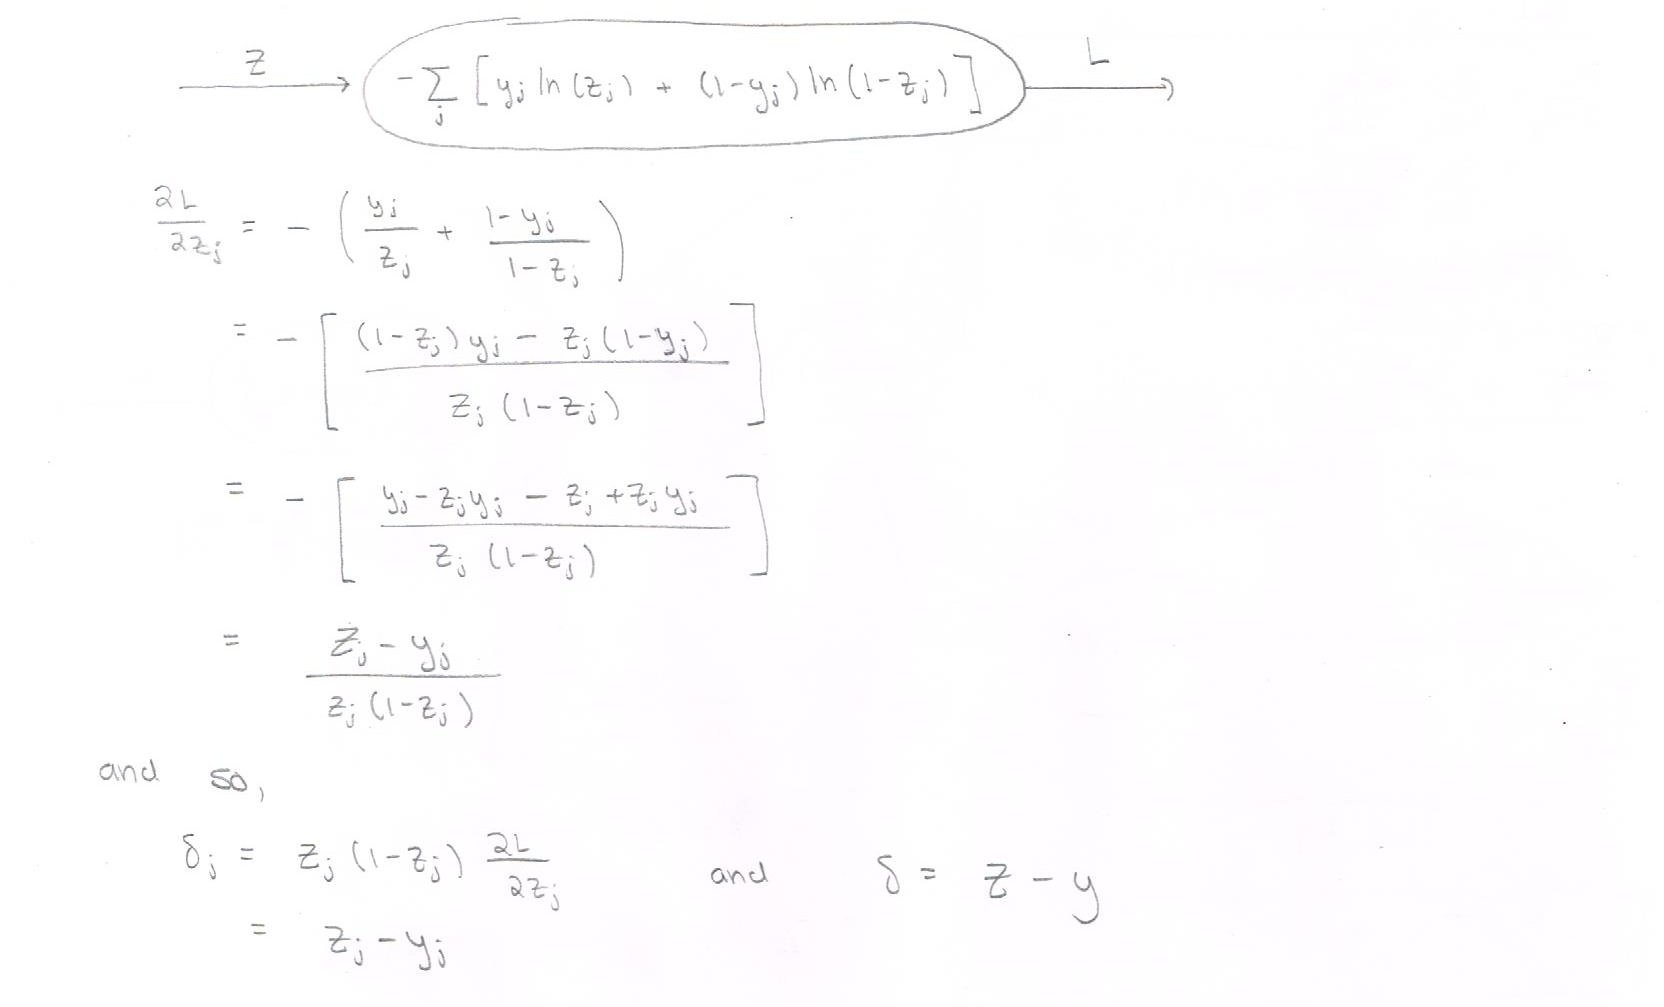
\includegraphics[scale=0.4]{002}
\end{center}

\section*{Problem 2}
\begin{enumerate}[a.]
  \item Mean-Squared Error
    \begin{itemize}
      \item All of the weights were initialized randomly, drawing from a normal distribution with a mean of 0 and a standard deviation of 0.01. A constant learning rate of 0.01 was used. Training was stopped after one epoch (50000 images drawn randomly with replacement).
      \item The training accuracy was \textbf{0.89872}. The validation accuracy was \textbf{0.8814}.
      \item The total training time was \textbf{839.56} seconds (14 minutes).
      \item Below is a plot of the batch MSE loss over the training period calculated for every 1000 samples trained on
        \begin{center}
          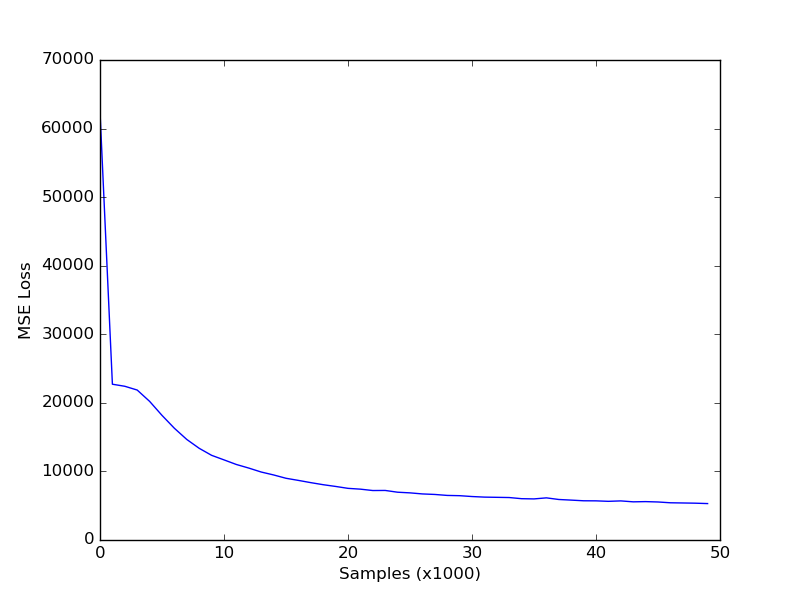
\includegraphics[scale=0.5]{mse_loss}
        \end{center}

        Below is a plot of the training accuracy over the training period.
        \begin{center}
          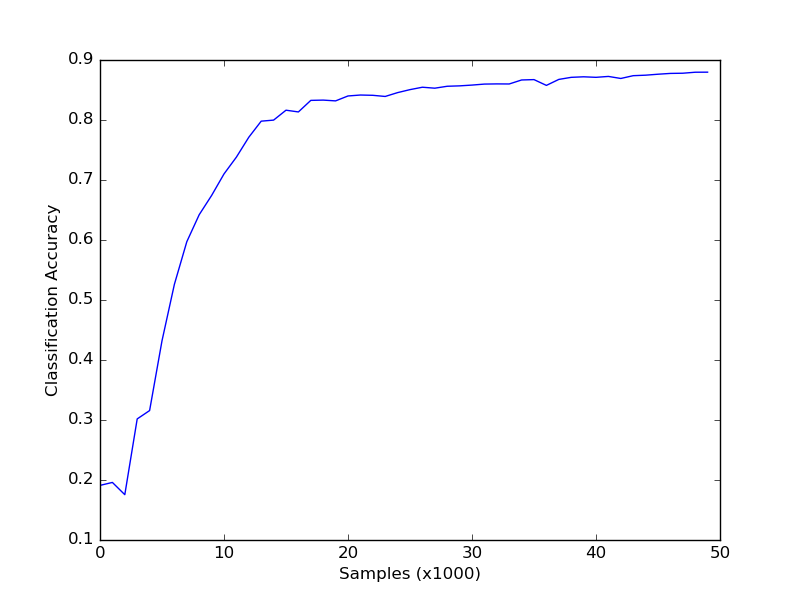
\includegraphics[scale=0.5]{mse_acc}
        \end{center}
        
    \end{itemize}

  \item Cross-Entropy Error
    \begin{itemize}
      \item All of the weights were initialized randomly, drawing from a normal distribution with a mean of 0 and a standard deviation of 0.01. A constant learning rate of 0.01 was used. Training was stopped after one epoch (50000 images drawn randomly with replacement).
      \item The final training accuracy was \textbf{0.9536}. The validation accuracy was \textbf{0.9412}.
      \item The total training time was \textbf{811.48} seconds (13.5 minutes).
      \item Below is a plot of the batch cross-entropy loss over the training period calculated for every 1000 samples trained on
        \begin{center}
          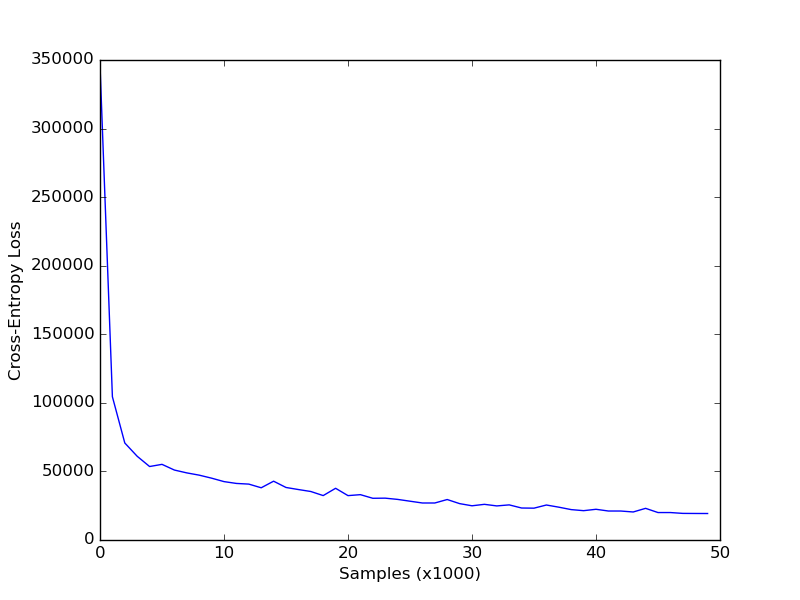
\includegraphics[scale=0.5]{ce_loss}
        \end{center}

        Below is a plot of the training accuracy over the training period.
        \begin{center}
          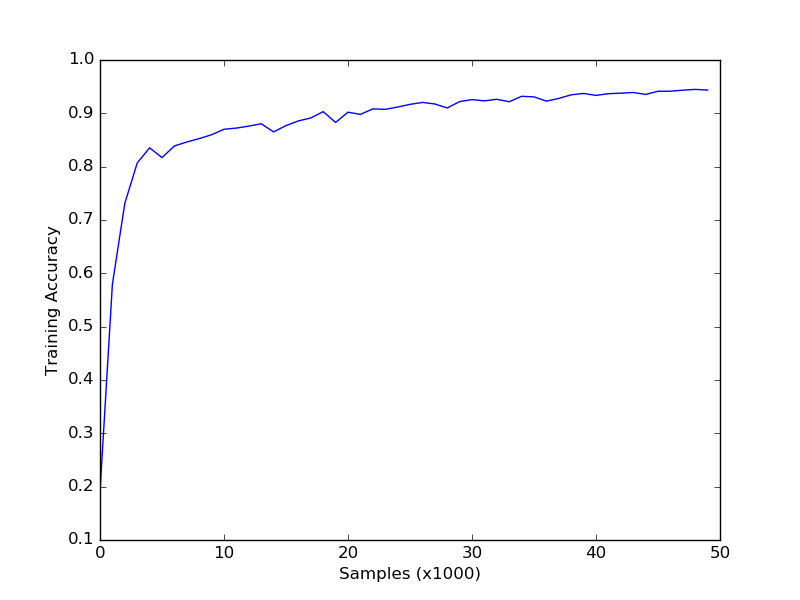
\includegraphics[scale=0.5]{ce_acc}
        \end{center}
        
    \end{itemize}

  \item From our results we see that the cross-entropy loss function performs considerably better than the mean-squared error. The difference in performance can be explained by examining their corresponing gradients with respect to the weight vectors, and in particular looking at the $\delta$ term that I define in my derivation above. For the mean-squared error,
    $$\delta = \left[z(1-z)\right](z-y)$$

    and for the cross-entropy error,
    $$\delta = z - y$$

    Where $z$ are our neural network outputs and $y$ are the true labels. We see that the mse $\delta$ contains (inside the brackets) the derivative of the sigmoid function, which approaches 0 when our outputs $z$ are close to 0 or 1. Therefore $\delta$ and consequently the gradients also approach 0 as $z$ gets close to 0 and 1. For these cases, learning is slow because our gradients are small. In contrast, the $\delta$ for the cross-entropy error does not suffer from this ``learning slowdown'' (I got the term from http://neuralnetworksanddeeplearning.com/chap3.html which provides a nice description of this phenomenon) and is strictly proportional to the error, which is what we would like because the more wrong we are, the larger our gradient and the more we learn.

  \item My best Kaggle score (after training for 10 epochs with 50000 images per epoch) was \textbf{0.97860}
\end{enumerate}


\end{document}
